\documentclass[tikz,border=0pt]{standalone}
\usepackage[american]{circuitikz}
\usetikzlibrary{arrows.meta,calc,positioning,decorations.pathmorphing,patterns}
\definecolor{zyloTeal}{HTML}{174A5B}
\definecolor{zyloTealTwo}{HTML}{246B7A}
\definecolor{zyloInk}{HTML}{1F2933}
\definecolor{zyloSoft}{HTML}{EAF4F4}
\definecolor{zyloPaper}{HTML}{F8FAFB}
\definecolor{zyloLine}{HTML}{44606B}
\definecolor{zyloOrange}{HTML}{D97706}
\begin{document}
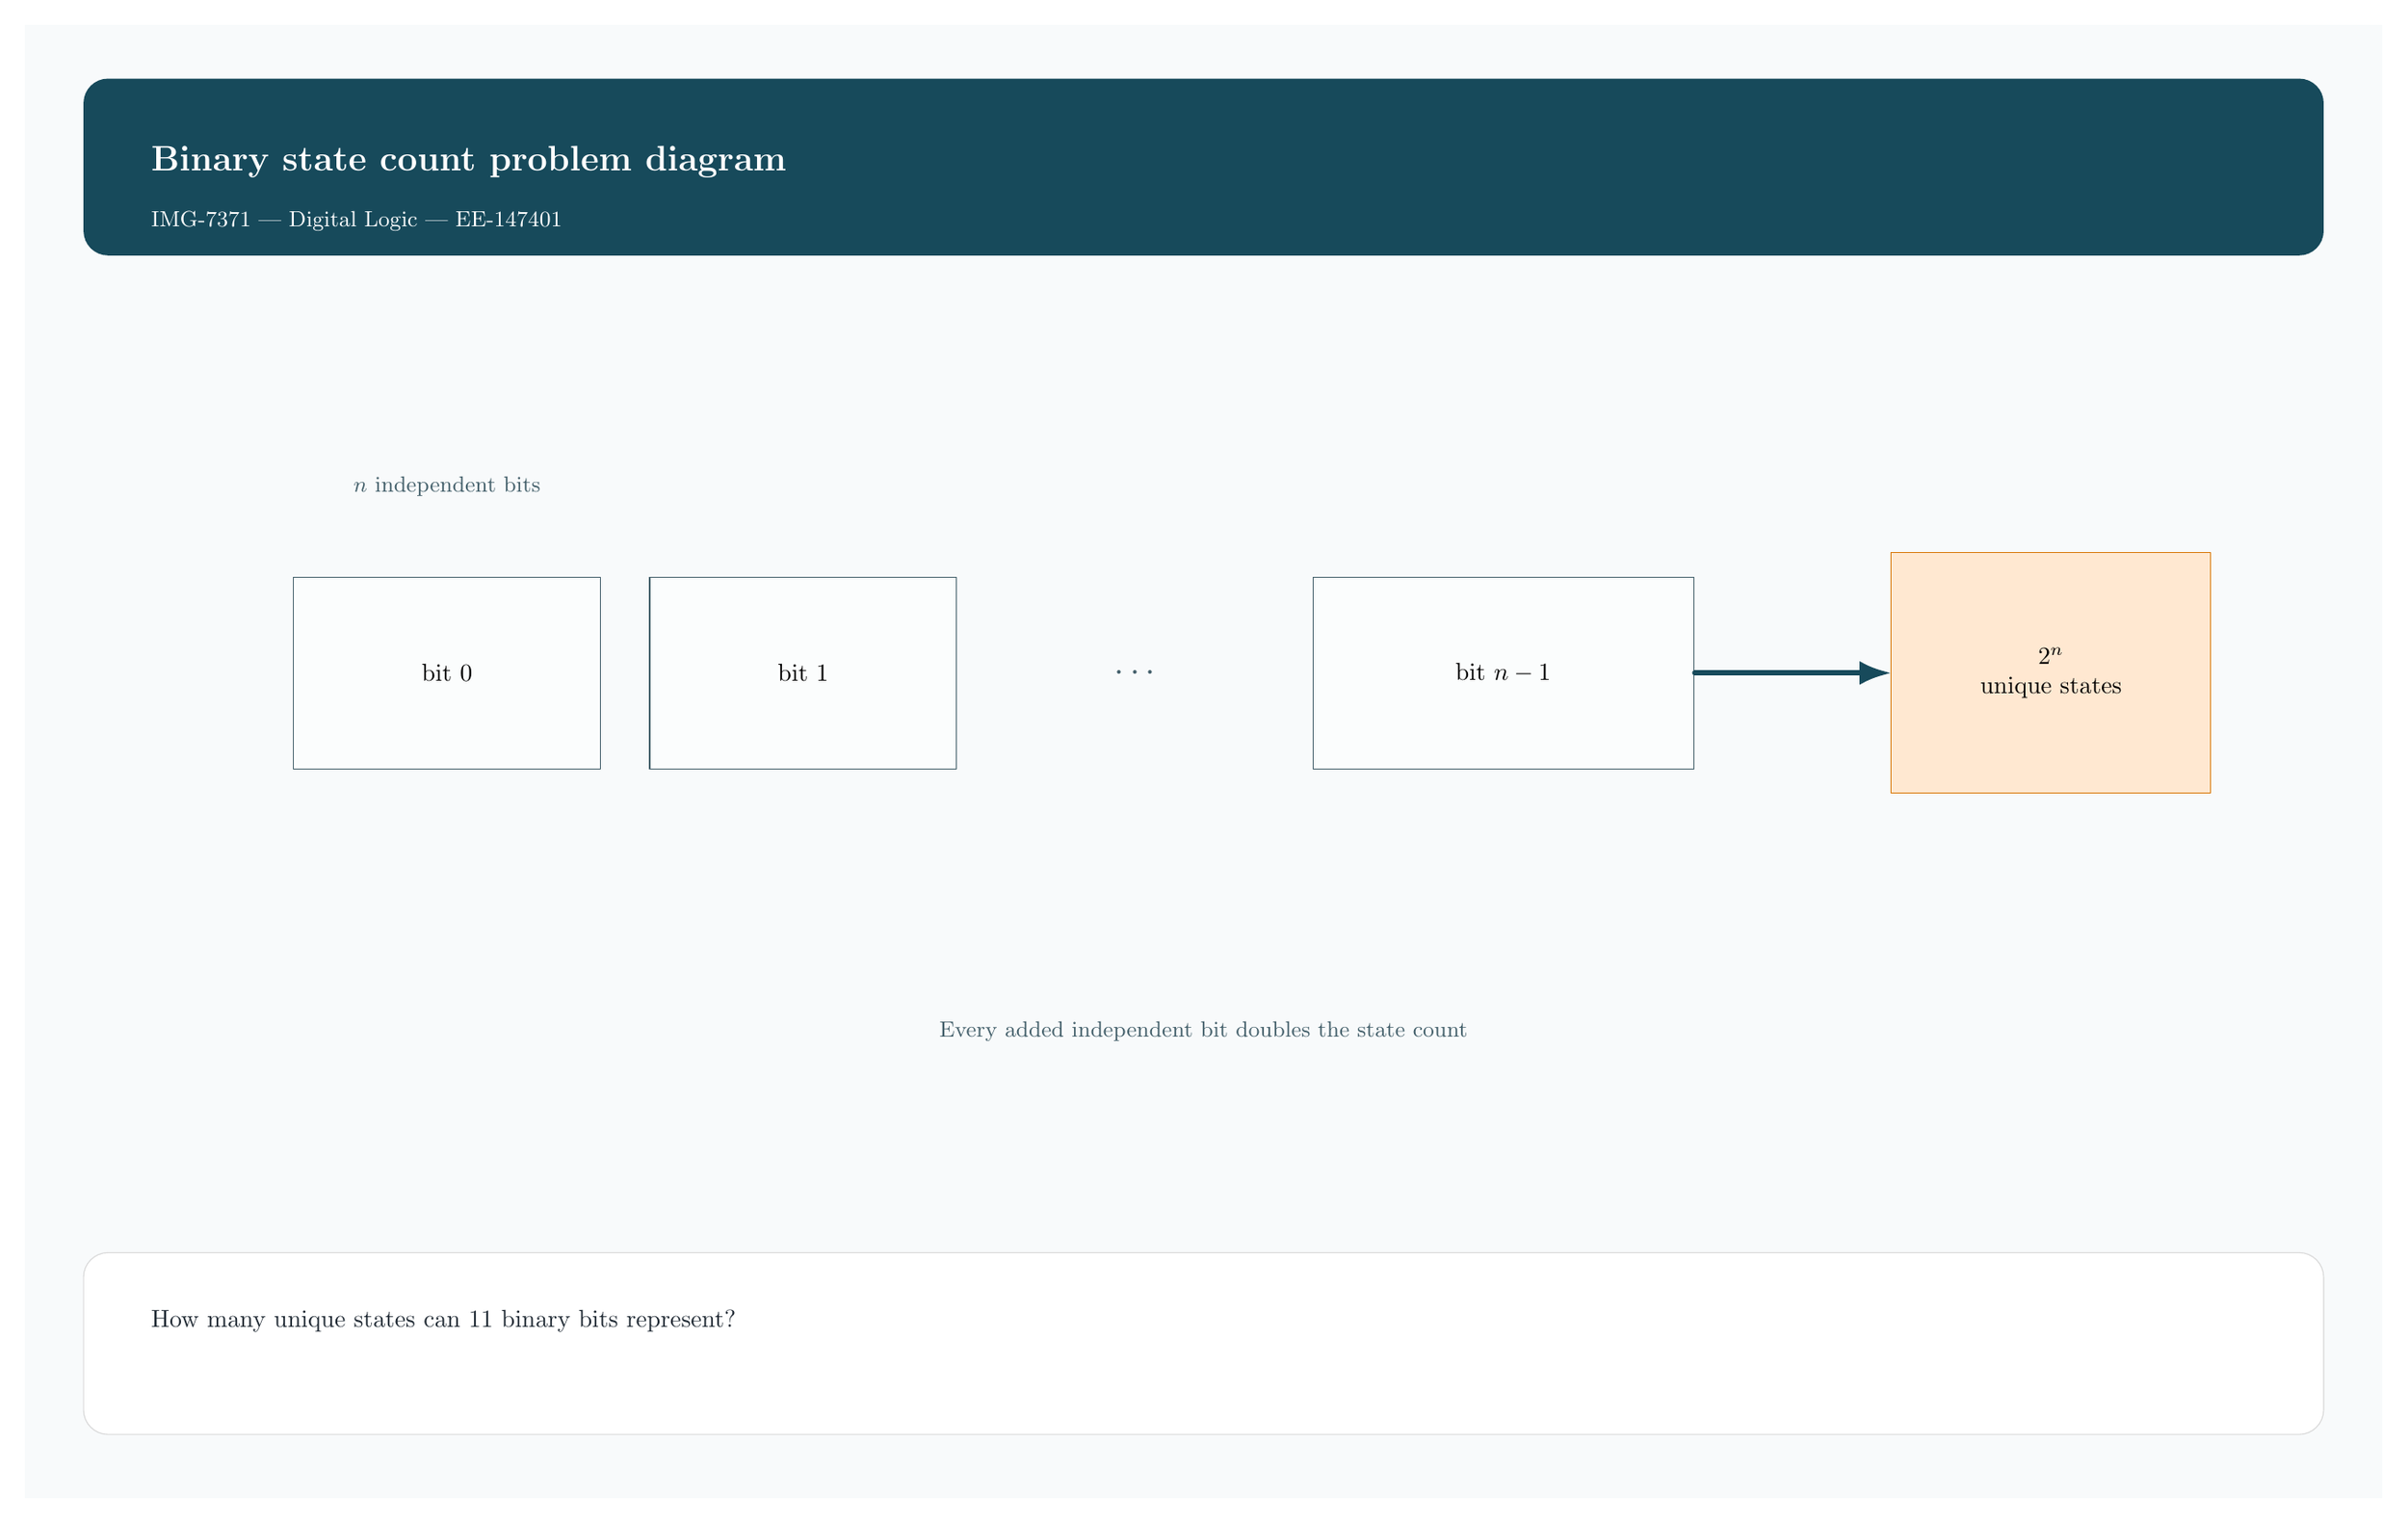
\begin{tikzpicture}[x=1pt,y=-1pt,>=Latex,line cap=round,line join=round]
\path[fill=zyloPaper] (0,0) rectangle (960,600);
\path[fill=zyloTeal,rounded corners=10pt] (24,22) rectangle (936,94);
\node[anchor=west,text=white,font=\bfseries\Large] at (48,56) {Binary state count problem diagram};
\node[anchor=west,text=white!82,font=\small] at (48,80) {IMG-7371 | Digital Logic | EE-147401};
\tikzset{wire/.style={draw=zyloTeal,line width=2.2pt},thinwire/.style={draw=zyloLine,line width=1.35pt},accent/.style={draw=zyloOrange,line width=2.2pt},box/.style={draw=zyloTealTwo,fill=zyloSoft,line width=1.5pt,rounded corners=8pt}}
\node[font=\small,text=zyloLine] at (172,188) {$n$ independent bits};
\node[draw=zyloLine,fill=white!80!zyloSoft,minimum width=125pt,minimum height=78pt] at (172,264) {bit 0};
\node[draw=zyloLine,fill=white!80!zyloSoft,minimum width=125pt,minimum height=78pt] at (317,264) {bit 1};
\node[font=\Large,text=zyloLine] at (452,264) {$\cdots$};
\node[draw=zyloLine,fill=white!80!zyloSoft,minimum width=155pt,minimum height=78pt] at (602,264) {bit $n-1$};
\draw[wire,->] (680,264) -- (760,264);
\node[draw=zyloOrange,fill=orange!18,minimum width=130pt,minimum height=98pt,align=center] at (825,264) {$2^n$\\unique states};
\node[font=\small,text=zyloLine] at (480,410) {Every added independent bit doubles the state count};
\path[draw=black!15,fill=white,rounded corners=10pt] (24,500) rectangle (936,574);
\node[anchor=west,text width=860pt,align=left,text=zyloInk,font=\normalsize] at (48,528) {How many unique states can 11 binary bits represent?};
\end{tikzpicture}
\end{document}
